% !TEX program = xelatex


\documentclass{resume}
\usepackage{zh_CN-Adobefonts_external}
\usepackage{linespacing_fix}
\usepackage{graphicx}
\usepackage{tabu}
\usepackage{multirow}
\usepackage{progressbar}
%\usepackage{zh_CN-Adobefonts_external} % Simplified Chinese Support using external fonts (./fonts/zh_CN-Adobe/)
%\usepackage{zh_CN-Adobefonts_internal} % Simplified Chinese Support using system fonts

\usepackage{tikz,xcolor,hyperref}
\usepackage{academicons}
\definecolor{orcidlogocol}{HTML}{A6CE39}

\definecolor{lime}{HTML}{A6CE39}
\DeclareRobustCommand{\orcidicon}{
	
\begin{tikzpicture}
	\draw[lime, fill=lime] (0,0) 
	circle [radius=0.16] 
	node[white] {{\fontfamily{qag}\selectfont \tiny ID}};
	\draw[white, fill=white] (-0.0625,0.095) 
	circle [radius=0.007];
	\end{tikzpicture}
	\hspace{-2mm}
}

\begin{document}
\pagenumbering{gobble} % suppress displaying page number

{\Large
  \begin{tabu}{ c l r }
    \multirow{5}{1in}{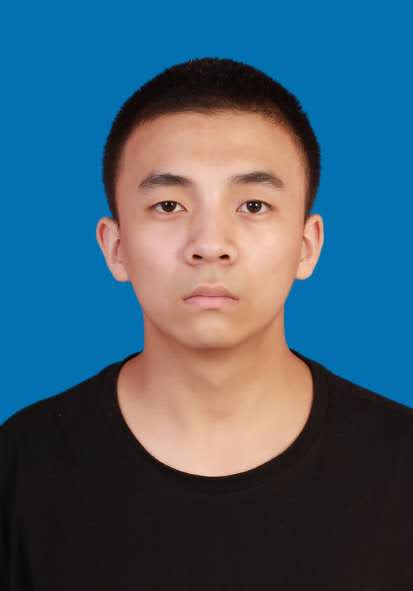
\includegraphics[width=0.88in]{avatar}} & \scshape{单子奇} & {Python~}\progressbar{0.8} \\
    & \email{breeze.shane@qq.com} & {Rust, C~}\progressbar{0.65} \\
    & \phone{(+86) 138-0423-2322} & {Linux~}\progressbar{0.6} \\
    % & \orcidicon\author[单子奇{\orcidauthorA{}}] & {Java, C++~}\progressbar{0.4} \\
    & \github[github.com/BreezeShane]{https://github.com/BreezeShane} & {Java, C++~}\progressbar{0.4} \\
    & \href{https://orcid.org/0009-0006-5493-7706}{\textcolor{orcidlogocol}{\aiOrcid} orcid.org/0009-0006-5493-7706} & {Lua, Shell~}\progressbar{0.3}
  \end{tabu}
}
 
\section{\faGraduationCap\  教育背景1}
\datedsubsection{\textbf{桂林电子科技大学}, 桂林}{2020年 -- 2024年}
\datedline{\textit{本科生}\ 软件工程专业}{2024 年 6 月}

\section{\faUsers\ 科研/项目经历}
\datedsubsection{\textbf{生成对抗网络论文研究与复现}}{2021年5月 -- 2022年10月}
\role{Python}{个人项目}
\begin{onehalfspacing}
研究与复现生成对抗网络项目, https://github.com/BreezeShane/Unsupervised-Learning
\begin{itemize}
  \item 复现了经典生成对抗网络Generative Adversaria Network
  \item 复现了WGAN以及其衍生版本WGAN-gp和WGAN-div
\end{itemize}
研究笔记: 
\begin{itemize}
  \item Generative Adversarial Networks: http://breezeshane.github.io/ArtificialIntelligence/GAN/StandardGAN/
  \item Wasserstein Generative Adversarial Networks: http://breezeshane.github.io/ArtificialIntelligence/GAN/WGAN/
  \item WGAN with Gradient Penalty: http://breezeshane.github.io/ArtificialIntelligence/GAN/WGAN-gp/
  \item Wasserstein Divergence for GANs: http://breezeshane.github.io/ArtificialIntelligence/GAN/WGAN-div/
\end{itemize}
\end{onehalfspacing}

\datedsubsection{\textbf{基于生成对抗网络的低照度增强系统}}{2021 年8月 -- 2022年10月}
\role{Python}{个人项目}
\begin{onehalfspacing}
参考论文实现完成的低照度增强系统, https://github.com/BreezeShane/NovelEnlightenGAN
\begin{itemize}
  \item 对原有项目进行精简化,去除冗余的代码
  \item 基于Flask框架完成前后端交互
  \item 对系统配置进行集中化处理,便于管理系统
\end{itemize}
\end{onehalfspacing}

\datedsubsection{\textbf{低照度增强测试评分系统}}{2021 年8月 -- 2022年10月}
\role{Python}{合作项目}
\begin{onehalfspacing}
小组合作的基于KinD的低照度增强系统的评分系统, https://github.com/BreezeShane/Metrics
\begin{itemize}
  \item 支持多种指标计算,如: MAE, MSE, PSNR, SSIM, LPIPS, NIQE, SPAQ, NIMA等
  \item 可移植性强
\end{itemize}
\end{onehalfspacing}

\datedsubsection{\textbf{微型图书管理系统}}{2022 年5月 -- 2022年6月}
\role{Shell, Python}{个人项目}
\begin{onehalfspacing}
面向中小型的图书管理系统, https://github.com/Tiny-LIMS-Team/LibraryInfoManager
\begin{itemize}
  \item 从设计到开发均由个人完成
  \item 基于Django框架开发的Web应用程序
  \item 使用MySQL数据库支持运行, 并通过 ORM 方式管理数据库
\end{itemize}
\end{onehalfspacing}

\datedsubsection{\textbf{云存储服务系统}}{2022年12月 -- 2023年1月}
\role{Vue, Python}{合作项目}
\begin{onehalfspacing}
多用户云存储服务系统后端开发, https://github.com/Tiny-LIMS-Team/HadoopNetDisk, 本人完成了整个项目的后端设计与业务逻辑功能,并参与实现了后端与集群的交互
\begin{itemize}
  \item 采用了JwT安全认证
  \item 基于Apache Hdfs文件系统、MySQL与HBase数据库完成开发
  \item 设计上采用 C-P-S 模式即客户端-代理-服务端进行服务支持
\end{itemize}
\end{onehalfspacing}

\datedsubsection{\textbf{DocScanner论文}}{2022 年6月 -- 2023年1月}
\role{\LaTeX}{合作项目}
\begin{onehalfspacing}
一篇基于语义分割的文档扫描系统论文, 发表于2022年第18届计算智能与安全国际会议(CIS)上, 本人为该论文的第一作者. \\
论文 DOI 为\href{https://doi.org/10.1109/CIS58238.2022.00028}{10.1109/CIS58238.2022.00028} \\
ISBN 信息: 
\begin{itemize}
\item Electronic ISBN: 979-8-3503-4627-5
\item Print on Demand(PoD) ISBN: 979-8-3503-4628-2
\end{itemize}
\end{onehalfspacing}

\datedsubsection{\textbf{基于C++\&Qt的音乐播放器}}{2023 年6月 -- 2023年7月}
\role{C++, Qt}{合作项目}
\begin{onehalfspacing}
基于C++和Qt实现的音乐播放器, https://github.com/BreezeShane/PineappleMusic, 本人完成其中歌词滚动与播放控制的功能。
% \begin{itemize}
% \item Electronic ISBN: 979-8-3503-4627-5
% \item Print on Demand(PoD) ISBN: 979-8-3503-4628-2
% \end{itemize}
\end{onehalfspacing}

% Reference Test
%\datedsubsection{\textbf{Paper Title\cite{zaharia2012resilient}}}{May. 2015}
%An xxx optimized for xxx\cite{verma2015large}
%\begin{itemize}
%  \item main contribution
%\end{itemize}

\section{\faCogs\ IT 技能}
% increase linespacing [parsep=0.5ex]
\begin{itemize}[parsep=0.5ex]
  \item 编程语言: Python > Rust $\approx$ C > C++ > Java > Lua
  \item 平台: Linux
  \item 框架: Django, PyTorch
\end{itemize}

\section{\faHeartO\ 获奖情况}
\datedline{\textit{企业命题类第三名}, 第十二届中国大学生服务外包创新创业大赛}{2021 年8 月}
\datedline{\textit{铜奖}, 第七届中国国际“互联网+”大学生创新创业大赛“数广集团杯”广西赛区}{2021 年8 月}
\datedline{\textit{}2021-2022学年度国家励志奖学金}{2022 年12 月}
\datedline{\textit{}2020-2021学年度国家励志奖学金}{2021 年12 月}

\section{\faInfo\ 其他}
% increase linespacing [parsep=0.5ex]
\begin{itemize}[parsep=0.5ex]
  \item 技术博客: http://breezeshane.github.io/
  \item GitHub: https://github.com/BreezeShane
  \item ORCID: https://orcid.org/0009-0006-5493-7706
  \item 语言: 英语 - 熟练(CET4 459.0)
\end{itemize}

%% Reference
%\newpage
%\bibliographystyle{IEEETran}
%\bibliography{mycite}
\end{document}
